% Created by tikzDevice version 0.12.6 on 2026-07-03 11:54:53
% !TEX encoding = UTF-8 Unicode
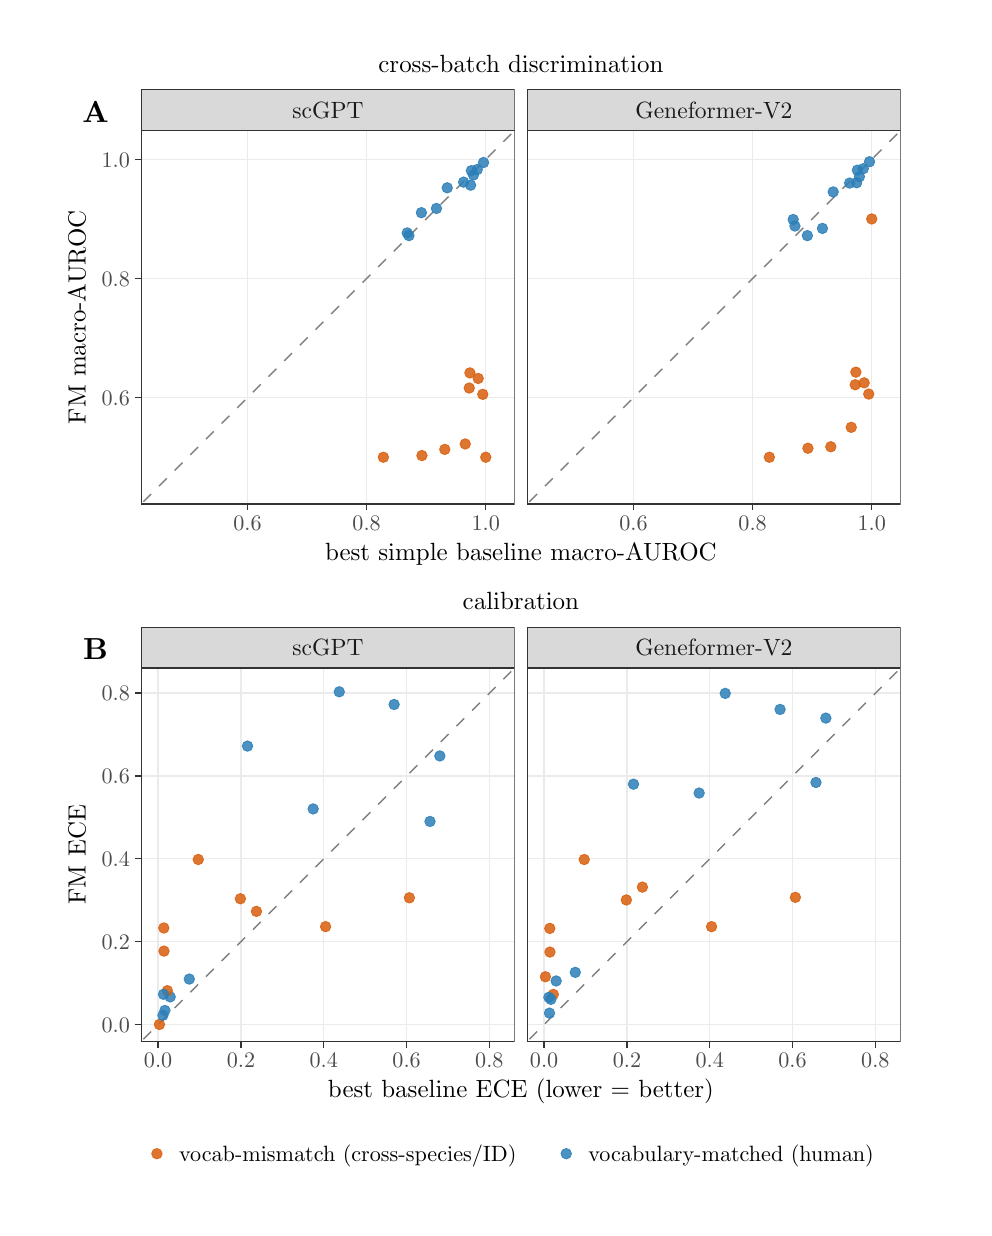
\begin{tikzpicture}[x=1pt,y=1pt]
\definecolor{fillColor}{RGB}{255,255,255}
\path[use as bounding box,fill=fillColor,fill opacity=0.00] (0,0) rectangle (338.22,426.39);
\begin{scope}
\path[clip] (  0.00,  0.00) rectangle (338.22,426.39);
\definecolor{drawColor}{RGB}{255,255,255}
\definecolor{fillColor}{RGB}{255,255,255}

\path[draw=drawColor,line width= 0.5pt,line join=round,line cap=round,fill=fillColor] ( -0.00, -0.00) rectangle (338.22,426.39);
\end{scope}
\begin{scope}
\path[clip] (  5.00,227.20) rectangle (329.22,421.39);
\definecolor{drawColor}{RGB}{255,255,255}
\definecolor{fillColor}{RGB}{255,255,255}

\path[draw=drawColor,line width= 0.5pt,line join=round,line cap=round,fill=fillColor] (  5.00,227.20) rectangle (329.22,421.39);
\end{scope}
\begin{scope}
\path[clip] (  5.00,  5.00) rectangle (329.22,227.20);
\definecolor{drawColor}{RGB}{255,255,255}
\definecolor{fillColor}{RGB}{255,255,255}

\path[draw=drawColor,line width= 0.5pt,line join=round,line cap=round,fill=fillColor] (  5.00,  5.00) rectangle (329.22,227.20);
\end{scope}
\begin{scope}
\path[clip] ( 41.00,254.26) rectangle (175.97,389.24);
\definecolor{fillColor}{RGB}{255,255,255}

\path[fill=fillColor] ( 41.00,254.26) rectangle (175.97,389.24);
\definecolor{drawColor}{gray}{0.92}

\path[draw=drawColor,line width= 0.5pt,line join=round] ( 41.00,292.69) --
	(175.97,292.69);

\path[draw=drawColor,line width= 0.5pt,line join=round] ( 41.00,335.74) --
	(175.97,335.74);

\path[draw=drawColor,line width= 0.5pt,line join=round] ( 41.00,378.79) --
	(175.97,378.79);

\path[draw=drawColor,line width= 0.5pt,line join=round] ( 79.43,254.26) --
	( 79.43,389.24);

\path[draw=drawColor,line width= 0.5pt,line join=round] (122.48,254.26) --
	(122.48,389.24);

\path[draw=drawColor,line width= 0.5pt,line join=round] (165.53,254.26) --
	(165.53,389.24);
\definecolor{drawColor}{gray}{0.50}

\path[draw=drawColor,line width= 0.5pt,dash pattern=on 4pt off 4pt ,line join=round] (-93.97,119.29) -- (310.94,524.21);
\definecolor{drawColor}{RGB}{44,127,184}
\definecolor{fillColor}{RGB}{44,127,184}

\path[draw=drawColor,draw opacity=0.85,line width= 0.3pt,line join=round,line cap=round,fill=fillColor,fill opacity=0.85] (161.07,373.14) circle (  1.90);

\path[draw=drawColor,draw opacity=0.85,line width= 0.3pt,line join=round,line cap=round,fill=fillColor,fill opacity=0.85] (137.77,351.24) circle (  1.90);
\definecolor{drawColor}{RGB}{217,95,14}
\definecolor{fillColor}{RGB}{217,95,14}

\path[draw=drawColor,draw opacity=0.85,line width= 0.3pt,line join=round,line cap=round,fill=fillColor,fill opacity=0.85] (159.56,296.17) circle (  1.90);
\definecolor{drawColor}{RGB}{44,127,184}
\definecolor{fillColor}{RGB}{44,127,184}

\path[draw=drawColor,draw opacity=0.85,line width= 0.3pt,line join=round,line cap=round,fill=fillColor,fill opacity=0.85] (137.14,352.22) circle (  1.90);

\path[draw=drawColor,draw opacity=0.85,line width= 0.3pt,line join=round,line cap=round,fill=fillColor,fill opacity=0.85] (147.71,361.06) circle (  1.90);
\definecolor{drawColor}{RGB}{217,95,14}
\definecolor{fillColor}{RGB}{217,95,14}

\path[draw=drawColor,draw opacity=0.85,line width= 0.3pt,line join=round,line cap=round,fill=fillColor,fill opacity=0.85] (159.80,301.64) circle (  1.90);
\definecolor{drawColor}{RGB}{44,127,184}
\definecolor{fillColor}{RGB}{44,127,184}

\path[draw=drawColor,draw opacity=0.85,line width= 0.3pt,line join=round,line cap=round,fill=fillColor,fill opacity=0.85] (160.06,369.47) circle (  1.90);
\definecolor{drawColor}{RGB}{217,95,14}
\definecolor{fillColor}{RGB}{217,95,14}

\path[draw=drawColor,draw opacity=0.85,line width= 0.3pt,line join=round,line cap=round,fill=fillColor,fill opacity=0.85] (162.79,299.63) circle (  1.90);
\definecolor{drawColor}{RGB}{44,127,184}
\definecolor{fillColor}{RGB}{44,127,184}

\path[draw=drawColor,draw opacity=0.85,line width= 0.3pt,line join=round,line cap=round,fill=fillColor,fill opacity=0.85] (151.60,368.52) circle (  1.90);

\path[draw=drawColor,draw opacity=0.85,line width= 0.3pt,line join=round,line cap=round,fill=fillColor,fill opacity=0.85] (142.27,359.53) circle (  1.90);

\path[draw=drawColor,draw opacity=0.85,line width= 0.3pt,line join=round,line cap=round,fill=fillColor,fill opacity=0.85] (160.33,374.72) circle (  1.90);

\path[draw=drawColor,draw opacity=0.85,line width= 0.3pt,line join=round,line cap=round,fill=fillColor,fill opacity=0.85] (157.53,370.57) circle (  1.90);
\definecolor{drawColor}{RGB}{217,95,14}
\definecolor{fillColor}{RGB}{217,95,14}

\path[draw=drawColor,draw opacity=0.85,line width= 0.3pt,line join=round,line cap=round,fill=fillColor,fill opacity=0.85] (165.53,271.16) circle (  1.90);

\path[draw=drawColor,draw opacity=0.85,line width= 0.3pt,line join=round,line cap=round,fill=fillColor,fill opacity=0.85] (128.53,271.16) circle (  1.90);

\path[draw=drawColor,draw opacity=0.85,line width= 0.3pt,line join=round,line cap=round,fill=fillColor,fill opacity=0.85] (158.11,275.96) circle (  1.90);
\definecolor{drawColor}{RGB}{44,127,184}
\definecolor{fillColor}{RGB}{44,127,184}

\path[draw=drawColor,draw opacity=0.85,line width= 0.3pt,line join=round,line cap=round,fill=fillColor,fill opacity=0.85] (164.72,377.66) circle (  1.90);
\definecolor{drawColor}{RGB}{217,95,14}
\definecolor{fillColor}{RGB}{217,95,14}

\path[draw=drawColor,draw opacity=0.85,line width= 0.3pt,line join=round,line cap=round,fill=fillColor,fill opacity=0.85] (150.73,274.00) circle (  1.90);
\definecolor{drawColor}{RGB}{44,127,184}
\definecolor{fillColor}{RGB}{44,127,184}

\path[draw=drawColor,draw opacity=0.85,line width= 0.3pt,line join=round,line cap=round,fill=fillColor,fill opacity=0.85] (162.47,375.14) circle (  1.90);
\definecolor{drawColor}{RGB}{217,95,14}
\definecolor{fillColor}{RGB}{217,95,14}

\path[draw=drawColor,draw opacity=0.85,line width= 0.3pt,line join=round,line cap=round,fill=fillColor,fill opacity=0.85] (164.45,293.89) circle (  1.90);

\path[draw=drawColor,draw opacity=0.85,line width= 0.3pt,line join=round,line cap=round,fill=fillColor,fill opacity=0.85] (142.46,271.77) circle (  1.90);
\definecolor{drawColor}{gray}{0.20}

\path[draw=drawColor,line width= 0.5pt,line join=round,line cap=round] ( 41.00,254.26) rectangle (175.97,389.24);
\end{scope}
\begin{scope}
\path[clip] (180.47,254.26) rectangle (315.44,389.24);
\definecolor{fillColor}{RGB}{255,255,255}

\path[fill=fillColor] (180.47,254.26) rectangle (315.44,389.24);
\definecolor{drawColor}{gray}{0.92}

\path[draw=drawColor,line width= 0.5pt,line join=round] (180.47,292.69) --
	(315.44,292.69);

\path[draw=drawColor,line width= 0.5pt,line join=round] (180.47,335.74) --
	(315.44,335.74);

\path[draw=drawColor,line width= 0.5pt,line join=round] (180.47,378.79) --
	(315.44,378.79);

\path[draw=drawColor,line width= 0.5pt,line join=round] (218.90,254.26) --
	(218.90,389.24);

\path[draw=drawColor,line width= 0.5pt,line join=round] (261.95,254.26) --
	(261.95,389.24);

\path[draw=drawColor,line width= 0.5pt,line join=round] (305.00,254.26) --
	(305.00,389.24);
\definecolor{drawColor}{gray}{0.50}

\path[draw=drawColor,line width= 0.5pt,dash pattern=on 4pt off 4pt ,line join=round] ( 45.50,119.29) -- (450.42,524.21);
\definecolor{drawColor}{RGB}{44,127,184}
\definecolor{fillColor}{RGB}{44,127,184}

\path[draw=drawColor,draw opacity=0.85,line width= 0.3pt,line join=round,line cap=round,fill=fillColor,fill opacity=0.85] (300.54,372.55) circle (  1.90);

\path[draw=drawColor,draw opacity=0.85,line width= 0.3pt,line join=round,line cap=round,fill=fillColor,fill opacity=0.85] (277.24,354.71) circle (  1.90);
\definecolor{drawColor}{RGB}{217,95,14}
\definecolor{fillColor}{RGB}{217,95,14}

\path[draw=drawColor,draw opacity=0.85,line width= 0.3pt,line join=round,line cap=round,fill=fillColor,fill opacity=0.85] (299.03,297.36) circle (  1.90);
\definecolor{drawColor}{RGB}{44,127,184}
\definecolor{fillColor}{RGB}{44,127,184}

\path[draw=drawColor,draw opacity=0.85,line width= 0.3pt,line join=round,line cap=round,fill=fillColor,fill opacity=0.85] (276.61,357.06) circle (  1.90);

\path[draw=drawColor,draw opacity=0.85,line width= 0.3pt,line join=round,line cap=round,fill=fillColor,fill opacity=0.85] (287.18,353.85) circle (  1.90);
\definecolor{drawColor}{RGB}{217,95,14}
\definecolor{fillColor}{RGB}{217,95,14}

\path[draw=drawColor,draw opacity=0.85,line width= 0.3pt,line join=round,line cap=round,fill=fillColor,fill opacity=0.85] (299.27,301.91) circle (  1.90);
\definecolor{drawColor}{RGB}{44,127,184}
\definecolor{fillColor}{RGB}{44,127,184}

\path[draw=drawColor,draw opacity=0.85,line width= 0.3pt,line join=round,line cap=round,fill=fillColor,fill opacity=0.85] (299.54,370.34) circle (  1.90);
\definecolor{drawColor}{RGB}{217,95,14}
\definecolor{fillColor}{RGB}{217,95,14}

\path[draw=drawColor,draw opacity=0.85,line width= 0.3pt,line join=round,line cap=round,fill=fillColor,fill opacity=0.85] (302.26,298.04) circle (  1.90);
\definecolor{drawColor}{RGB}{44,127,184}
\definecolor{fillColor}{RGB}{44,127,184}

\path[draw=drawColor,draw opacity=0.85,line width= 0.3pt,line join=round,line cap=round,fill=fillColor,fill opacity=0.85] (291.07,367.04) circle (  1.90);

\path[draw=drawColor,draw opacity=0.85,line width= 0.3pt,line join=round,line cap=round,fill=fillColor,fill opacity=0.85] (281.74,351.24) circle (  1.90);

\path[draw=drawColor,draw opacity=0.85,line width= 0.3pt,line join=round,line cap=round,fill=fillColor,fill opacity=0.85] (299.81,374.89) circle (  1.90);

\path[draw=drawColor,draw opacity=0.85,line width= 0.3pt,line join=round,line cap=round,fill=fillColor,fill opacity=0.85] (297.00,370.23) circle (  1.90);
\definecolor{drawColor}{RGB}{217,95,14}
\definecolor{fillColor}{RGB}{217,95,14}

\path[draw=drawColor,draw opacity=0.85,line width= 0.3pt,line join=round,line cap=round,fill=fillColor,fill opacity=0.85] (305.00,357.26) circle (  1.90);

\path[draw=drawColor,draw opacity=0.85,line width= 0.3pt,line join=round,line cap=round,fill=fillColor,fill opacity=0.85] (268.00,271.16) circle (  1.90);

\path[draw=drawColor,draw opacity=0.85,line width= 0.3pt,line join=round,line cap=round,fill=fillColor,fill opacity=0.85] (297.59,281.97) circle (  1.90);
\definecolor{drawColor}{RGB}{44,127,184}
\definecolor{fillColor}{RGB}{44,127,184}

\path[draw=drawColor,draw opacity=0.85,line width= 0.3pt,line join=round,line cap=round,fill=fillColor,fill opacity=0.85] (304.19,377.94) circle (  1.90);
\definecolor{drawColor}{RGB}{217,95,14}
\definecolor{fillColor}{RGB}{217,95,14}

\path[draw=drawColor,draw opacity=0.85,line width= 0.3pt,line join=round,line cap=round,fill=fillColor,fill opacity=0.85] (290.21,274.95) circle (  1.90);
\definecolor{drawColor}{RGB}{44,127,184}
\definecolor{fillColor}{RGB}{44,127,184}

\path[draw=drawColor,draw opacity=0.85,line width= 0.3pt,line join=round,line cap=round,fill=fillColor,fill opacity=0.85] (301.94,375.42) circle (  1.90);
\definecolor{drawColor}{RGB}{217,95,14}
\definecolor{fillColor}{RGB}{217,95,14}

\path[draw=drawColor,draw opacity=0.85,line width= 0.3pt,line join=round,line cap=round,fill=fillColor,fill opacity=0.85] (303.92,293.98) circle (  1.90);

\path[draw=drawColor,draw opacity=0.85,line width= 0.3pt,line join=round,line cap=round,fill=fillColor,fill opacity=0.85] (281.94,274.41) circle (  1.90);
\definecolor{drawColor}{gray}{0.20}

\path[draw=drawColor,line width= 0.5pt,line join=round,line cap=round] (180.47,254.26) rectangle (315.44,389.24);
\end{scope}
\begin{scope}
\path[clip] (  0.00,  0.00) rectangle (338.22,426.39);
\definecolor{drawColor}{RGB}{0,0,0}

\node[text=drawColor,anchor=base,inner sep=0pt, outer sep=0pt, scale=  1.10] at ( 24.53,392.14) {\bfseries A};
\end{scope}
\begin{scope}
\path[clip] (  0.00,  0.00) rectangle (338.22,426.39);
\definecolor{drawColor}{gray}{0.30}

\node[text=drawColor,anchor=base east,inner sep=0pt, outer sep=0pt, scale=  0.80] at ( 36.95,289.93) {0.6};

\node[text=drawColor,anchor=base east,inner sep=0pt, outer sep=0pt, scale=  0.80] at ( 36.95,332.99) {0.8};

\node[text=drawColor,anchor=base east,inner sep=0pt, outer sep=0pt, scale=  0.80] at ( 36.95,376.04) {1.0};
\end{scope}
\begin{scope}
\path[clip] (  0.00,  0.00) rectangle (338.22,426.39);
\definecolor{drawColor}{gray}{0.20}

\path[draw=drawColor,line width= 0.5pt,line join=round] ( 38.75,292.69) --
	( 41.00,292.69);

\path[draw=drawColor,line width= 0.5pt,line join=round] ( 38.75,335.74) --
	( 41.00,335.74);

\path[draw=drawColor,line width= 0.5pt,line join=round] ( 38.75,378.79) --
	( 41.00,378.79);
\end{scope}
\begin{scope}
\path[clip] (  0.00,  0.00) rectangle (338.22,426.39);
\definecolor{drawColor}{RGB}{0,0,0}

\node[text=drawColor,rotate= 90.00,anchor=base,inner sep=0pt, outer sep=0pt, scale=  0.90] at ( 20.98,321.75) {FM macro-AUROC};
\end{scope}
\begin{scope}
\path[clip] ( 41.00,389.24) rectangle (175.97,403.94);
\definecolor{drawColor}{gray}{0.20}
\definecolor{fillColor}{gray}{0.85}

\path[draw=drawColor,line width= 0.5pt,line join=round,line cap=round,fill=fillColor] ( 41.00,389.24) rectangle (175.97,403.94);
\definecolor{drawColor}{gray}{0.10}

\node[text=drawColor,anchor=base,inner sep=0pt, outer sep=0pt, scale=  0.85] at (108.49,393.66) {scGPT};
\end{scope}
\begin{scope}
\path[clip] (180.47,389.24) rectangle (315.44,403.94);
\definecolor{drawColor}{gray}{0.20}
\definecolor{fillColor}{gray}{0.85}

\path[draw=drawColor,line width= 0.5pt,line join=round,line cap=round,fill=fillColor] (180.47,389.24) rectangle (315.44,403.94);
\definecolor{drawColor}{gray}{0.10}

\node[text=drawColor,anchor=base,inner sep=0pt, outer sep=0pt, scale=  0.85] at (247.96,393.66) {Geneformer-V2};
\end{scope}
\begin{scope}
\path[clip] (  0.00,  0.00) rectangle (338.22,426.39);
\definecolor{drawColor}{gray}{0.20}

\path[draw=drawColor,line width= 0.5pt,line join=round] ( 79.43,252.01) --
	( 79.43,254.26);

\path[draw=drawColor,line width= 0.5pt,line join=round] (122.48,252.01) --
	(122.48,254.26);

\path[draw=drawColor,line width= 0.5pt,line join=round] (165.53,252.01) --
	(165.53,254.26);
\end{scope}
\begin{scope}
\path[clip] (  0.00,  0.00) rectangle (338.22,426.39);
\definecolor{drawColor}{gray}{0.30}

\node[text=drawColor,anchor=base,inner sep=0pt, outer sep=0pt, scale=  0.80] at ( 79.43,244.70) {0.6};

\node[text=drawColor,anchor=base,inner sep=0pt, outer sep=0pt, scale=  0.80] at (122.48,244.70) {0.8};

\node[text=drawColor,anchor=base,inner sep=0pt, outer sep=0pt, scale=  0.80] at (165.53,244.70) {1.0};
\end{scope}
\begin{scope}
\path[clip] (  0.00,  0.00) rectangle (338.22,426.39);
\definecolor{drawColor}{gray}{0.20}

\path[draw=drawColor,line width= 0.5pt,line join=round] (218.90,252.01) --
	(218.90,254.26);

\path[draw=drawColor,line width= 0.5pt,line join=round] (261.95,252.01) --
	(261.95,254.26);

\path[draw=drawColor,line width= 0.5pt,line join=round] (305.00,252.01) --
	(305.00,254.26);
\end{scope}
\begin{scope}
\path[clip] (  0.00,  0.00) rectangle (338.22,426.39);
\definecolor{drawColor}{gray}{0.30}

\node[text=drawColor,anchor=base,inner sep=0pt, outer sep=0pt, scale=  0.80] at (218.90,244.70) {0.6};

\node[text=drawColor,anchor=base,inner sep=0pt, outer sep=0pt, scale=  0.80] at (261.95,244.70) {0.8};

\node[text=drawColor,anchor=base,inner sep=0pt, outer sep=0pt, scale=  0.80] at (305.00,244.70) {1.0};
\end{scope}
\begin{scope}
\path[clip] (  0.00,  0.00) rectangle (338.22,426.39);
\definecolor{drawColor}{RGB}{0,0,0}

\node[text=drawColor,anchor=base,inner sep=0pt, outer sep=0pt, scale=  0.90] at (178.22,233.95) {best simple baseline macro-AUROC};
\end{scope}
\begin{scope}
\path[clip] (  0.00,  0.00) rectangle (338.22,426.39);
\definecolor{drawColor}{RGB}{0,0,0}

\node[text=drawColor,anchor=base,inner sep=0pt, outer sep=0pt, scale=  0.90] at (178.22,410.19) {cross-batch discrimination};
\end{scope}
\begin{scope}
\path[clip] ( 41.00, 60.07) rectangle (175.97,195.04);
\definecolor{fillColor}{RGB}{255,255,255}

\path[fill=fillColor] ( 41.00, 60.07) rectangle (175.97,195.04);
\definecolor{drawColor}{gray}{0.92}

\path[draw=drawColor,line width= 0.5pt,line join=round] ( 41.00, 66.20) --
	(175.97, 66.20);

\path[draw=drawColor,line width= 0.5pt,line join=round] ( 41.00, 96.13) --
	(175.97, 96.13);

\path[draw=drawColor,line width= 0.5pt,line join=round] ( 41.00,126.06) --
	(175.97,126.06);

\path[draw=drawColor,line width= 0.5pt,line join=round] ( 41.00,155.98) --
	(175.97,155.98);

\path[draw=drawColor,line width= 0.5pt,line join=round] ( 41.00,185.91) --
	(175.97,185.91);

\path[draw=drawColor,line width= 0.5pt,line join=round] ( 47.14, 60.07) --
	( 47.14,195.04);

\path[draw=drawColor,line width= 0.5pt,line join=round] ( 77.06, 60.07) --
	( 77.06,195.04);

\path[draw=drawColor,line width= 0.5pt,line join=round] (106.99, 60.07) --
	(106.99,195.04);

\path[draw=drawColor,line width= 0.5pt,line join=round] (136.92, 60.07) --
	(136.92,195.04);

\path[draw=drawColor,line width= 0.5pt,line join=round] (166.84, 60.07) --
	(166.84,195.04);
\definecolor{drawColor}{gray}{0.50}

\path[draw=drawColor,line width= 0.5pt,dash pattern=on 4pt off 4pt ,line join=round] (-93.97,-74.91) -- (310.94,330.01);
\definecolor{drawColor}{RGB}{44,127,184}
\definecolor{fillColor}{RGB}{44,127,184}

\path[draw=drawColor,draw opacity=0.85,line width= 0.3pt,line join=round,line cap=round,fill=fillColor,fill opacity=0.85] ( 51.49, 76.17) circle (  1.90);

\path[draw=drawColor,draw opacity=0.85,line width= 0.3pt,line join=round,line cap=round,fill=fillColor,fill opacity=0.85] (145.38,139.56) circle (  1.90);
\definecolor{drawColor}{RGB}{217,95,14}
\definecolor{fillColor}{RGB}{217,95,14}

\path[draw=drawColor,draw opacity=0.85,line width= 0.3pt,line join=round,line cap=round,fill=fillColor,fill opacity=0.85] ( 50.47, 78.41) circle (  1.90);
\definecolor{drawColor}{RGB}{44,127,184}
\definecolor{fillColor}{RGB}{44,127,184}

\path[draw=drawColor,draw opacity=0.85,line width= 0.3pt,line join=round,line cap=round,fill=fillColor,fill opacity=0.85] (112.59,186.40) circle (  1.90);

\path[draw=drawColor,draw opacity=0.85,line width= 0.3pt,line join=round,line cap=round,fill=fillColor,fill opacity=0.85] (132.41,181.82) circle (  1.90);
\definecolor{drawColor}{RGB}{217,95,14}
\definecolor{fillColor}{RGB}{217,95,14}

\path[draw=drawColor,draw opacity=0.85,line width= 0.3pt,line join=round,line cap=round,fill=fillColor,fill opacity=0.85] ( 76.86,111.62) circle (  1.90);
\definecolor{drawColor}{RGB}{44,127,184}
\definecolor{fillColor}{RGB}{44,127,184}

\path[draw=drawColor,draw opacity=0.85,line width= 0.3pt,line join=round,line cap=round,fill=fillColor,fill opacity=0.85] (103.16,144.08) circle (  1.90);
\definecolor{drawColor}{RGB}{217,95,14}
\definecolor{fillColor}{RGB}{217,95,14}

\path[draw=drawColor,draw opacity=0.85,line width= 0.3pt,line join=round,line cap=round,fill=fillColor,fill opacity=0.85] ( 82.66,107.07) circle (  1.90);
\definecolor{drawColor}{RGB}{44,127,184}
\definecolor{fillColor}{RGB}{44,127,184}

\path[draw=drawColor,draw opacity=0.85,line width= 0.3pt,line join=round,line cap=round,fill=fillColor,fill opacity=0.85] ( 79.43,166.79) circle (  1.90);

\path[draw=drawColor,draw opacity=0.85,line width= 0.3pt,line join=round,line cap=round,fill=fillColor,fill opacity=0.85] (148.94,163.23) circle (  1.90);

\path[draw=drawColor,draw opacity=0.85,line width= 0.3pt,line join=round,line cap=round,fill=fillColor,fill opacity=0.85] ( 49.09, 77.10) circle (  1.90);

\path[draw=drawColor,draw opacity=0.85,line width= 0.3pt,line join=round,line cap=round,fill=fillColor,fill opacity=0.85] ( 58.40, 82.60) circle (  1.90);
\definecolor{drawColor}{RGB}{217,95,14}
\definecolor{fillColor}{RGB}{217,95,14}

\path[draw=drawColor,draw opacity=0.85,line width= 0.3pt,line join=round,line cap=round,fill=fillColor,fill opacity=0.85] ( 47.61, 66.20) circle (  1.90);

\path[draw=drawColor,draw opacity=0.85,line width= 0.3pt,line join=round,line cap=round,fill=fillColor,fill opacity=0.85] ( 61.64,125.81) circle (  1.90);

\path[draw=drawColor,draw opacity=0.85,line width= 0.3pt,line join=round,line cap=round,fill=fillColor,fill opacity=0.85] ( 49.19,101.06) circle (  1.90);
\definecolor{drawColor}{RGB}{44,127,184}
\definecolor{fillColor}{RGB}{44,127,184}

\path[draw=drawColor,draw opacity=0.85,line width= 0.3pt,line join=round,line cap=round,fill=fillColor,fill opacity=0.85] ( 49.59, 71.25) circle (  1.90);
\definecolor{drawColor}{RGB}{217,95,14}
\definecolor{fillColor}{RGB}{217,95,14}

\path[draw=drawColor,draw opacity=0.85,line width= 0.3pt,line join=round,line cap=round,fill=fillColor,fill opacity=0.85] (107.65,101.55) circle (  1.90);
\definecolor{drawColor}{RGB}{44,127,184}
\definecolor{fillColor}{RGB}{44,127,184}

\path[draw=drawColor,draw opacity=0.85,line width= 0.3pt,line join=round,line cap=round,fill=fillColor,fill opacity=0.85] ( 48.86, 69.49) circle (  1.90);
\definecolor{drawColor}{RGB}{217,95,14}
\definecolor{fillColor}{RGB}{217,95,14}

\path[draw=drawColor,draw opacity=0.85,line width= 0.3pt,line join=round,line cap=round,fill=fillColor,fill opacity=0.85] ( 49.25, 92.70) circle (  1.90);

\path[draw=drawColor,draw opacity=0.85,line width= 0.3pt,line join=round,line cap=round,fill=fillColor,fill opacity=0.85] (137.93,111.97) circle (  1.90);
\definecolor{drawColor}{gray}{0.20}

\path[draw=drawColor,line width= 0.5pt,line join=round,line cap=round] ( 41.00, 60.07) rectangle (175.97,195.04);
\end{scope}
\begin{scope}
\path[clip] (180.47, 60.07) rectangle (315.44,195.04);
\definecolor{fillColor}{RGB}{255,255,255}

\path[fill=fillColor] (180.47, 60.07) rectangle (315.44,195.04);
\definecolor{drawColor}{gray}{0.92}

\path[draw=drawColor,line width= 0.5pt,line join=round] (180.47, 66.20) --
	(315.44, 66.20);

\path[draw=drawColor,line width= 0.5pt,line join=round] (180.47, 96.13) --
	(315.44, 96.13);

\path[draw=drawColor,line width= 0.5pt,line join=round] (180.47,126.06) --
	(315.44,126.06);

\path[draw=drawColor,line width= 0.5pt,line join=round] (180.47,155.98) --
	(315.44,155.98);

\path[draw=drawColor,line width= 0.5pt,line join=round] (180.47,185.91) --
	(315.44,185.91);

\path[draw=drawColor,line width= 0.5pt,line join=round] (186.61, 60.07) --
	(186.61,195.04);

\path[draw=drawColor,line width= 0.5pt,line join=round] (216.54, 60.07) --
	(216.54,195.04);

\path[draw=drawColor,line width= 0.5pt,line join=round] (246.46, 60.07) --
	(246.46,195.04);

\path[draw=drawColor,line width= 0.5pt,line join=round] (276.39, 60.07) --
	(276.39,195.04);

\path[draw=drawColor,line width= 0.5pt,line join=round] (306.32, 60.07) --
	(306.32,195.04);
\definecolor{drawColor}{gray}{0.50}

\path[draw=drawColor,line width= 0.5pt,dash pattern=on 4pt off 4pt ,line join=round] ( 45.50,-74.91) -- (450.42,330.01);
\definecolor{drawColor}{RGB}{44,127,184}
\definecolor{fillColor}{RGB}{44,127,184}

\path[draw=drawColor,draw opacity=0.85,line width= 0.3pt,line join=round,line cap=round,fill=fillColor,fill opacity=0.85] (190.96, 81.92) circle (  1.90);

\path[draw=drawColor,draw opacity=0.85,line width= 0.3pt,line join=round,line cap=round,fill=fillColor,fill opacity=0.85] (284.85,153.63) circle (  1.90);
\definecolor{drawColor}{RGB}{217,95,14}
\definecolor{fillColor}{RGB}{217,95,14}

\path[draw=drawColor,draw opacity=0.85,line width= 0.3pt,line join=round,line cap=round,fill=fillColor,fill opacity=0.85] (189.94, 77.06) circle (  1.90);
\definecolor{drawColor}{RGB}{44,127,184}
\definecolor{fillColor}{RGB}{44,127,184}

\path[draw=drawColor,draw opacity=0.85,line width= 0.3pt,line join=round,line cap=round,fill=fillColor,fill opacity=0.85] (252.06,185.83) circle (  1.90);

\path[draw=drawColor,draw opacity=0.85,line width= 0.3pt,line join=round,line cap=round,fill=fillColor,fill opacity=0.85] (271.88,180.03) circle (  1.90);
\definecolor{drawColor}{RGB}{217,95,14}
\definecolor{fillColor}{RGB}{217,95,14}

\path[draw=drawColor,draw opacity=0.85,line width= 0.3pt,line join=round,line cap=round,fill=fillColor,fill opacity=0.85] (216.33,111.19) circle (  1.90);
\definecolor{drawColor}{RGB}{44,127,184}
\definecolor{fillColor}{RGB}{44,127,184}

\path[draw=drawColor,draw opacity=0.85,line width= 0.3pt,line join=round,line cap=round,fill=fillColor,fill opacity=0.85] (242.63,149.82) circle (  1.90);
\definecolor{drawColor}{RGB}{217,95,14}
\definecolor{fillColor}{RGB}{217,95,14}

\path[draw=drawColor,draw opacity=0.85,line width= 0.3pt,line join=round,line cap=round,fill=fillColor,fill opacity=0.85] (222.13,115.83) circle (  1.90);
\definecolor{drawColor}{RGB}{44,127,184}
\definecolor{fillColor}{RGB}{44,127,184}

\path[draw=drawColor,draw opacity=0.85,line width= 0.3pt,line join=round,line cap=round,fill=fillColor,fill opacity=0.85] (218.91,153.03) circle (  1.90);

\path[draw=drawColor,draw opacity=0.85,line width= 0.3pt,line join=round,line cap=round,fill=fillColor,fill opacity=0.85] (288.42,176.90) circle (  1.90);

\path[draw=drawColor,draw opacity=0.85,line width= 0.3pt,line join=round,line cap=round,fill=fillColor,fill opacity=0.85] (188.56, 70.30) circle (  1.90);

\path[draw=drawColor,draw opacity=0.85,line width= 0.3pt,line join=round,line cap=round,fill=fillColor,fill opacity=0.85] (197.87, 85.02) circle (  1.90);
\definecolor{drawColor}{RGB}{217,95,14}
\definecolor{fillColor}{RGB}{217,95,14}

\path[draw=drawColor,draw opacity=0.85,line width= 0.3pt,line join=round,line cap=round,fill=fillColor,fill opacity=0.85] (187.08, 83.43) circle (  1.90);

\path[draw=drawColor,draw opacity=0.85,line width= 0.3pt,line join=round,line cap=round,fill=fillColor,fill opacity=0.85] (201.11,125.81) circle (  1.90);

\path[draw=drawColor,draw opacity=0.85,line width= 0.3pt,line join=round,line cap=round,fill=fillColor,fill opacity=0.85] (188.67,100.91) circle (  1.90);
\definecolor{drawColor}{RGB}{44,127,184}
\definecolor{fillColor}{RGB}{44,127,184}

\path[draw=drawColor,draw opacity=0.85,line width= 0.3pt,line join=round,line cap=round,fill=fillColor,fill opacity=0.85] (189.06, 75.28) circle (  1.90);
\definecolor{drawColor}{RGB}{217,95,14}
\definecolor{fillColor}{RGB}{217,95,14}

\path[draw=drawColor,draw opacity=0.85,line width= 0.3pt,line join=round,line cap=round,fill=fillColor,fill opacity=0.85] (247.12,101.54) circle (  1.90);
\definecolor{drawColor}{RGB}{44,127,184}
\definecolor{fillColor}{RGB}{44,127,184}

\path[draw=drawColor,draw opacity=0.85,line width= 0.3pt,line join=round,line cap=round,fill=fillColor,fill opacity=0.85] (188.33, 76.02) circle (  1.90);
\definecolor{drawColor}{RGB}{217,95,14}
\definecolor{fillColor}{RGB}{217,95,14}

\path[draw=drawColor,draw opacity=0.85,line width= 0.3pt,line join=round,line cap=round,fill=fillColor,fill opacity=0.85] (188.72, 92.36) circle (  1.90);

\path[draw=drawColor,draw opacity=0.85,line width= 0.3pt,line join=round,line cap=round,fill=fillColor,fill opacity=0.85] (277.40,112.13) circle (  1.90);
\definecolor{drawColor}{gray}{0.20}

\path[draw=drawColor,line width= 0.5pt,line join=round,line cap=round] (180.47, 60.07) rectangle (315.44,195.04);
\end{scope}
\begin{scope}
\path[clip] (  0.00,  0.00) rectangle (338.22,426.39);
\definecolor{drawColor}{RGB}{0,0,0}

\node[text=drawColor,anchor=base,inner sep=0pt, outer sep=0pt, scale=  1.10] at ( 24.53,197.94) {\bfseries B};
\end{scope}
\begin{scope}
\path[clip] (  0.00,  0.00) rectangle (338.22,426.39);
\definecolor{drawColor}{gray}{0.30}

\node[text=drawColor,anchor=base east,inner sep=0pt, outer sep=0pt, scale=  0.80] at ( 36.95, 63.45) {0.0};

\node[text=drawColor,anchor=base east,inner sep=0pt, outer sep=0pt, scale=  0.80] at ( 36.95, 93.37) {0.2};

\node[text=drawColor,anchor=base east,inner sep=0pt, outer sep=0pt, scale=  0.80] at ( 36.95,123.30) {0.4};

\node[text=drawColor,anchor=base east,inner sep=0pt, outer sep=0pt, scale=  0.80] at ( 36.95,153.23) {0.6};

\node[text=drawColor,anchor=base east,inner sep=0pt, outer sep=0pt, scale=  0.80] at ( 36.95,183.16) {0.8};
\end{scope}
\begin{scope}
\path[clip] (  0.00,  0.00) rectangle (338.22,426.39);
\definecolor{drawColor}{gray}{0.20}

\path[draw=drawColor,line width= 0.5pt,line join=round] ( 38.75, 66.20) --
	( 41.00, 66.20);

\path[draw=drawColor,line width= 0.5pt,line join=round] ( 38.75, 96.13) --
	( 41.00, 96.13);

\path[draw=drawColor,line width= 0.5pt,line join=round] ( 38.75,126.06) --
	( 41.00,126.06);

\path[draw=drawColor,line width= 0.5pt,line join=round] ( 38.75,155.98) --
	( 41.00,155.98);

\path[draw=drawColor,line width= 0.5pt,line join=round] ( 38.75,185.91) --
	( 41.00,185.91);
\end{scope}
\begin{scope}
\path[clip] (  0.00,  0.00) rectangle (338.22,426.39);
\definecolor{drawColor}{RGB}{0,0,0}

\node[text=drawColor,rotate= 90.00,anchor=base,inner sep=0pt, outer sep=0pt, scale=  0.90] at ( 20.98,127.55) {FM ECE};
\end{scope}
\begin{scope}
\path[clip] ( 41.00,195.04) rectangle (175.97,209.75);
\definecolor{drawColor}{gray}{0.20}
\definecolor{fillColor}{gray}{0.85}

\path[draw=drawColor,line width= 0.5pt,line join=round,line cap=round,fill=fillColor] ( 41.00,195.04) rectangle (175.97,209.75);
\definecolor{drawColor}{gray}{0.10}

\node[text=drawColor,anchor=base,inner sep=0pt, outer sep=0pt, scale=  0.85] at (108.49,199.46) {scGPT};
\end{scope}
\begin{scope}
\path[clip] (180.47,195.04) rectangle (315.44,209.75);
\definecolor{drawColor}{gray}{0.20}
\definecolor{fillColor}{gray}{0.85}

\path[draw=drawColor,line width= 0.5pt,line join=round,line cap=round,fill=fillColor] (180.47,195.04) rectangle (315.44,209.75);
\definecolor{drawColor}{gray}{0.10}

\node[text=drawColor,anchor=base,inner sep=0pt, outer sep=0pt, scale=  0.85] at (247.96,199.46) {Geneformer-V2};
\end{scope}
\begin{scope}
\path[clip] (  0.00,  0.00) rectangle (338.22,426.39);
\definecolor{drawColor}{gray}{0.20}

\path[draw=drawColor,line width= 0.5pt,line join=round] ( 47.14, 57.82) --
	( 47.14, 60.07);

\path[draw=drawColor,line width= 0.5pt,line join=round] ( 77.06, 57.82) --
	( 77.06, 60.07);

\path[draw=drawColor,line width= 0.5pt,line join=round] (106.99, 57.82) --
	(106.99, 60.07);

\path[draw=drawColor,line width= 0.5pt,line join=round] (136.92, 57.82) --
	(136.92, 60.07);

\path[draw=drawColor,line width= 0.5pt,line join=round] (166.84, 57.82) --
	(166.84, 60.07);
\end{scope}
\begin{scope}
\path[clip] (  0.00,  0.00) rectangle (338.22,426.39);
\definecolor{drawColor}{gray}{0.30}

\node[text=drawColor,anchor=base,inner sep=0pt, outer sep=0pt, scale=  0.80] at ( 47.14, 50.51) {0.0};

\node[text=drawColor,anchor=base,inner sep=0pt, outer sep=0pt, scale=  0.80] at ( 77.06, 50.51) {0.2};

\node[text=drawColor,anchor=base,inner sep=0pt, outer sep=0pt, scale=  0.80] at (106.99, 50.51) {0.4};

\node[text=drawColor,anchor=base,inner sep=0pt, outer sep=0pt, scale=  0.80] at (136.92, 50.51) {0.6};

\node[text=drawColor,anchor=base,inner sep=0pt, outer sep=0pt, scale=  0.80] at (166.84, 50.51) {0.8};
\end{scope}
\begin{scope}
\path[clip] (  0.00,  0.00) rectangle (338.22,426.39);
\definecolor{drawColor}{gray}{0.20}

\path[draw=drawColor,line width= 0.5pt,line join=round] (186.61, 57.82) --
	(186.61, 60.07);

\path[draw=drawColor,line width= 0.5pt,line join=round] (216.54, 57.82) --
	(216.54, 60.07);

\path[draw=drawColor,line width= 0.5pt,line join=round] (246.46, 57.82) --
	(246.46, 60.07);

\path[draw=drawColor,line width= 0.5pt,line join=round] (276.39, 57.82) --
	(276.39, 60.07);

\path[draw=drawColor,line width= 0.5pt,line join=round] (306.32, 57.82) --
	(306.32, 60.07);
\end{scope}
\begin{scope}
\path[clip] (  0.00,  0.00) rectangle (338.22,426.39);
\definecolor{drawColor}{gray}{0.30}

\node[text=drawColor,anchor=base,inner sep=0pt, outer sep=0pt, scale=  0.80] at (186.61, 50.51) {0.0};

\node[text=drawColor,anchor=base,inner sep=0pt, outer sep=0pt, scale=  0.80] at (216.54, 50.51) {0.2};

\node[text=drawColor,anchor=base,inner sep=0pt, outer sep=0pt, scale=  0.80] at (246.46, 50.51) {0.4};

\node[text=drawColor,anchor=base,inner sep=0pt, outer sep=0pt, scale=  0.80] at (276.39, 50.51) {0.6};

\node[text=drawColor,anchor=base,inner sep=0pt, outer sep=0pt, scale=  0.80] at (306.32, 50.51) {0.8};
\end{scope}
\begin{scope}
\path[clip] (  0.00,  0.00) rectangle (338.22,426.39);
\definecolor{drawColor}{RGB}{0,0,0}

\node[text=drawColor,anchor=base,inner sep=0pt, outer sep=0pt, scale=  0.90] at (178.22, 39.75) {best baseline ECE (lower = better)};
\end{scope}
\begin{scope}
\path[clip] (  0.00,  0.00) rectangle (338.22,426.39);
\definecolor{drawColor}{RGB}{0,0,0}

\node[text=drawColor,anchor=base,inner sep=0pt, outer sep=0pt, scale=  0.90] at (178.22,216.00) {calibration};
\end{scope}
\begin{scope}
\path[clip] (  0.00,  0.00) rectangle (338.22,426.39);
\definecolor{fillColor}{RGB}{255,255,255}

\path[fill=fillColor] ( 37.20, 10.00) rectangle (319.25, 29.00);
\end{scope}
\begin{scope}
\path[clip] (  0.00,  0.00) rectangle (338.22,426.39);
\definecolor{fillColor}{RGB}{255,255,255}

\path[fill=fillColor] ( 41.70, 14.50) rectangle ( 51.70, 24.50);
\definecolor{drawColor}{RGB}{217,95,14}
\definecolor{fillColor}{RGB}{217,95,14}

\path[draw=drawColor,draw opacity=0.85,line width= 0.3pt,line join=round,line cap=round,fill=fillColor,fill opacity=0.85] ( 46.70, 19.50) circle (  1.90);
\end{scope}
\begin{scope}
\path[clip] (  0.00,  0.00) rectangle (338.22,426.39);
\definecolor{fillColor}{RGB}{255,255,255}

\path[fill=fillColor] (189.61, 14.50) rectangle (199.61, 24.50);
\definecolor{drawColor}{RGB}{44,127,184}
\definecolor{fillColor}{RGB}{44,127,184}

\path[draw=drawColor,draw opacity=0.85,line width= 0.3pt,line join=round,line cap=round,fill=fillColor,fill opacity=0.85] (194.61, 19.50) circle (  1.90);
\end{scope}
\begin{scope}
\path[clip] (  0.00,  0.00) rectangle (338.22,426.39);
\definecolor{drawColor}{RGB}{0,0,0}

\node[text=drawColor,anchor=base west,inner sep=0pt, outer sep=0pt, scale=  0.80] at ( 54.70, 16.74) {vocab-mismatch (cross-species/ID)};
\end{scope}
\begin{scope}
\path[clip] (  0.00,  0.00) rectangle (338.22,426.39);
\definecolor{drawColor}{RGB}{0,0,0}

\node[text=drawColor,anchor=base west,inner sep=0pt, outer sep=0pt, scale=  0.80] at (202.61, 16.74) {vocabulary-matched (human)};
\end{scope}
\end{tikzpicture}
